\section{Method}
\label{sec:method}

\paragraph{Notation.}
We denote the number of transformer layers by~$N$, the sequence length by~$L$, and the number of selected tokens per query by~$k$.
At layer~$\ell$, the lightning indexer produces a score vector~$\mathbf{I}^{(\ell)}_{t} \in \mathbb{R}^{L}$ for query position~$t$, from which the top-$k$ index set~$\mathcal{T}^{(\ell)}_t = \mathrm{Top\text{-}k}(\mathbf{I}^{(\ell)}_t)$ is extracted ($k=2048$ throughout this paper).
We write~$\mathbf{p}^{(\ell)}_{t}$ for the aggregated attention distribution at layer~$\ell$ for position $t$ (obtained by averaging softmax attention weights across heads), and~$\mathbf{q}^{(\ell)}_t = \mathrm{Softmax}(\mathbf{I}^{(\ell)}_t)$ for the indexer's output distribution.

\paragraph{Overview.}
IndexCache modifies DSA by partitioning the~$N$ layers into two roles, encoded as a binary \emph{pattern string}~$\mathbf{c} = c_1 c_2 \cdots c_N$ with~$c_\ell \in \{\texttt{F}, \texttt{S}\}$:
\begin{itemize}[leftmargin=*,itemsep=2pt]
    \item \texttt{F}~(\textbf{Full}): the layer retains its indexer, computes fresh~$\mathcal{T}^{(\ell)}_t$ over all preceding tokens, and performs sparse core attention on the selected subset, identical to standard DSA.
    \item \texttt{S}~(\textbf{Shared}): the layer has \emph{no indexer}. It inherits the index set from the nearest preceding~\texttt{F}~layer, \emph{i.e.}\@\xspace, $\mathcal{T}^{(\ell)}_t \leftarrow \mathcal{T}^{(f(\ell))}_t$ where~$f(\ell) = \max\{j < \ell : c_j = \texttt{F}\}$, and directly applies sparse core attention using those inherited indices.
\end{itemize}
The first layer is always~\texttt{F} to seed the initial indices.
At inference, an~\texttt{S}~layer simply skips the indexer forward pass and reuses the cached index tensor from its~\texttt{F}~predecessor.
Figure~\ref{fig:pseudocode-comparison} illustrates the simplicity of this modification: the only change to the per-layer inference loop is a single conditional branch that either runs the indexer or copies the cached indices.

The key design question is how to choose the pattern~$\mathbf{c}$.
If most layers can safely share indices, a large fraction of the~$O(NL^2)$ total indexer cost can be eliminated while the~$O(NLk)$ core attention remains unchanged.
We propose two approaches: a \emph{training-free} method that determines~$\mathbf{c}$ via greedy search on an established DSA model~(Section~\ref{sec:method-trainfree}), and a \emph{training-aware} method that jointly optimizes the indexer parameters for cross-layer sharing via a multi-layer distillation loss~(Section~\ref{sec:method-trainaware}).

%% ============================================================
\subsection{Training-Free IndexCache}
\label{sec:method-trainfree}

Given a pretrained DSA model, our goal is to find a pattern~$\mathbf{c}$ that maximizes the number of~\texttt{S}~layers while minimizing the impact on model quality.
We first discuss why the most obvious approach fails, then present our greedy search algorithm.

\subsubsection{Why Uniform Interleaving Is Suboptimal}
\label{sec:method-interleave}

The simplest strategy is uniform interleaving: retain every~$r$-th layer's indexer and skip the rest (e.g., \texttt{FSSSFSSS}\dots for~$r{=}4$).
However, this ignores the fact that indexer importance varies significantly across layers.
We observe empirically that certain layers, particularly those in the early and transitional regions of the network, are far more sensitive to indexer removal than others.
Uniform interleaving may remove a critical indexer while retaining a redundant one, leading to noticeable quality degradation (see Section~\ref{sec:exp-trainfree} for quantitative comparisons).
This motivates a data-driven approach: let the model itself tell us which indexers are expendable, leading to our greedy layer selection algorithm.

\begin{algorithm}[t]
\caption{Greedy Layer Selection for Training-Free IndexCache}
\label{alg:greedy}
\begin{algorithmic}[1]
\REQUIRE DSA model~$M$ with~$N$ layers, calibration batches~$\mathcal{D}$, target \#~of~\texttt{S}~layers~$K$
\ENSURE Optimized pattern~$\mathbf{c}^*$
\STATE $\mathbf{c} \leftarrow \texttt{F}^N$ \hfill $\triangleright$~Initialize all layers as Full
\STATE $\mathcal{R} \leftarrow \{2, 3, \ldots, N\}$ \hfill $\triangleright$~Candidates (layer~1 always~\texttt{F})
\FOR{$\mathrm{step} = 1$ \TO $K$}
    \STATE $\ell^* \leftarrow \arg\min_{\ell \in \mathcal{R}} \;\textproc{EvalLoss}\bigl(M,\, \mathcal{D},\, \mathbf{c}|_{c_\ell \to \texttt{S}}\bigr)$
    \STATE $c_{\ell^*} \leftarrow \texttt{S}$,\; $\mathcal{R} \leftarrow \mathcal{R} \setminus \{\ell^*\}$
\ENDFOR
\RETURN $\mathbf{c}$
\end{algorithmic}
\end{algorithm}

\subsubsection{Layer Selection Algorithm}
\label{sec:method-greedy}

We propose a greedy search that incrementally converts~\texttt{F}~layers to~\texttt{S}~layers, using language modeling loss on a small calibration set as a proxy for downstream quality.

\paragraph{Calibration set.}
We cache~$B$ mini-batches from the training data.
All candidate patterns are evaluated on exactly the same batches, ensuring that loss differences reflect only the effect of the pattern change, not data variance. The loss is derived from a forward pass on the whole batch $\mathcal{D}$: $\textproc{EvalLoss}\bigl(M,\, \mathcal{D},\, \mathbf{c}\bigl)$.

\paragraph{Search procedure.}
Starting from the all-\texttt{F} baseline~($c_\ell = \texttt{F}$ for all~$\ell$), the algorithm proceeds for~$K$ steps, where~$K$ is the target number of~\texttt{S}~layers (e.g., $K = 3N/4$ to retain only~$1/4$ of indexers).
At each step, we iterate over all currently-\texttt{F} layers (excluding the first layer), tentatively flip each to~\texttt{S}, evaluate the resulting LM loss, and commit the flip that yields the lowest loss.
Algorithm~\ref{alg:greedy} presents the full procedure.

\paragraph{Complexity.}
A full search from all-\texttt{F} to all-\texttt{S} performs~$N(N{-}1)/2$ forward passes.
When pipeline parallelism partitions the model into~$P$ stages, we accelerate the search by splitting layers into~$P$ blocks (with each block's first layer fixed as~\texttt{F}) and searching blocks sequentially within each step: the best flip in each block is committed before the next block is searched, so that up to~$P$ layers are placed per step and total forward passes are reduced by roughly~$P{\times}$.


\begin{wrapfigure}{r}{0.35\linewidth}
    \centering
    \vspace{-1em}
    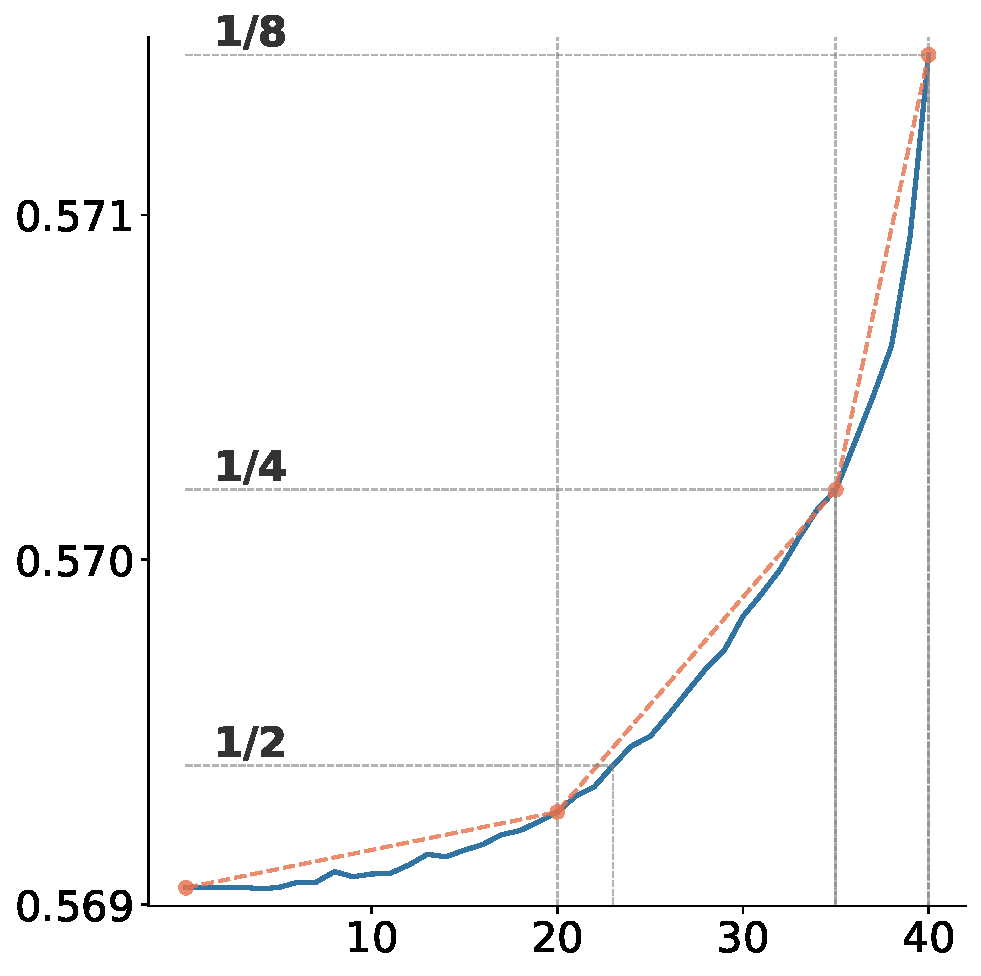
\includegraphics[width=\linewidth]{figures/search_simple.pdf}
    \vspace{-4em}
\end{wrapfigure}
\paragraph{Properties of the greedy solution.}
Although greedy search does not guarantee global optimality, we consistently observe three satisfying properties:
\begin{enumerate}[leftmargin=*,itemsep=1pt,label=(\arabic*)]
    \item The searched pattern outperforms uniform interleaving at the same retention ratio (Table~\ref{tab:trainfree}).
    \item As shown in the right figure (the steps for the 1/2, 1/4, and 1/8 retention ratios are marked), the per-step LM validation loss curve reveals a clear separation between ``easy'' layers (the first 20 steps) and ``critical'' layers (after 35 steps), suggesting a natural ordering of indexer importance.
    \item Results are stable across different calibration sets, indicating that this importance ranking is an intrinsic model property rather than a data artifact. Moreover, the LM loss serves as a valid proxy for downstream tasks, as lower LM loss is positively correlated with better task performance.
\end{enumerate}


\subsection{Training-Aware IndexCache with Multi-Layer Distillation}
\label{sec:method-trainaware}

Training-free IndexCache requires no weight updates, but is limited by the fact that each indexer was originally trained to serve only its own layer.
When training a DSA model from scratch or via continued pre-training, we can do better: explicitly training each retained indexer to serve \emph{multiple} layers simultaneously.

\paragraph{From single-layer to multi-layer distillation.}
In standard DSA training~(Section~\ref{sec:bg-dsa}), each indexer at layer~$\ell$ is distilled via KL divergence against its own layer's aggregated attention distribution~$\mathbf{p}^{(\ell)}_t$: $\mathcal{L}^{\mathrm{I}}
    = \sum_{t} D_{\mathrm{KL}}\!\left(
        \mathbf{p}^{(\ell)}_{t} \,\big\|\, \mathbf{q}^{(\ell)}_t
      \right)$.
We generalize this to a multi-layer objective.
Let layer~$\ell$ be a retained~\texttt{F}~layer, and let layers~$\ell{+}1, \ldots, \ell{+}m$ be the subsequent~\texttt{S}~layers that will reuse its index set~$\mathcal{T}^{(\ell)}_t$.
The multi-layer distillation loss is:
{\footnotesize
\begin{equation}
    \mathcal{L}^{\mathrm{I}}_{\mathrm{multi}}
    = \sum_{j=0}^{m} \frac{1}{m+1}\sum_{t}
      D_{\mathrm{KL}}\!\left(
        \mathbf{p}^{(\ell+j)}_{t} \,\big\|\, \mathbf{q}^{(\ell)}_t
      \right),
    \label{eq:multi-distill}
\end{equation}
}

Intuitively, this encourages the indexer to predict a top-$k$ set that is jointly useful for all layers it serves, rather than overfitting to layer~$\ell$ alone.

\paragraph{Gradient equivalence to distillation against the averaged distribution.}
A natural concern is whether optimizing a sum of KL terms introduces unexpected interactions.
We show that the multi-layer loss has a clean interpretation: it produces \emph{exactly the same gradient} as distilling against a single averaged target.

Define the averaged target~$\bar{\mathbf{p}}_{t} = \sum_{j=0}^{m} \frac{1}{m+1}\mathbf{p}^{(\ell+j)}_{t}$ and the corresponding single-target loss:
{\footnotesize
\begin{equation}
    \mathcal{L}^{\mathrm{I}}_{\mathrm{avg}}
    = \sum_{t} D_{\mathrm{KL}}\!\left(
        \bar{\mathbf{p}}_{t} \,\big\|\, \mathbf{q}^{(\ell)}_t
      \right).
    \label{eq:avg-distill}
\end{equation}
}

\begin{proposition}
\label{prop:grad-equiv}
$\nabla_\theta \mathcal{L}^{\mathrm{I}}_{\mathrm{multi}} = \nabla_\theta \mathcal{L}^{\mathrm{I}}_{\mathrm{avg}}$.
\end{proposition}

%\paragraph{Proof.}
\begin{proof}
Since~$\mathbf{q}^{(\ell)}_t$ is the only parameter-dependent term in~$D_{\mathrm{KL}}(\mathbf{p} \| \mathbf{q}^{(\ell)}_t)$, the entropy of~$\mathbf{p}$ vanishes under differentiation:
$\nabla_\theta D_{\mathrm{KL}}(\mathbf{p} \| \mathbf{q}^{(\ell)}_t) = -\nabla_\theta \sum_{s} \mathbf{p}(s) \log \mathbf{q}^{(\ell)}_t(s)$.
Apply to Eq.~\ref{eq:multi-distill}:
{\footnotesize
\begin{align}
    \nabla_\theta \, \mathcal{L}^{\mathrm{I}}_{\mathrm{multi}}
    &= -\sum_{j=0}^{m} \frac{1}{m+1} \sum_{t} \nabla_\theta \sum_{s} \mathbf{p}^{(\ell+j)}_{t}(s) \log \mathbf{q}^{(\ell)}_t(s) \notag \\
    &= -\sum_{t} \nabla_\theta \sum_{s} \underbrace{\Bigl(\textstyle\sum_{j=0}^{m} \frac{1}{m+1} \mathbf{p}^{(\ell+j)}_{t}(s)\Bigr)}_{\bar{\mathbf{p}}_{t}(s)} \log \mathbf{q}^{(\ell)}_t(s)
    \;=\; \nabla_\theta \, \mathcal{L}^{\mathrm{I}}_{\mathrm{avg}}.
    \label{eq:grad-equiv-proof}
\end{align}
}
\end{proof}

\paragraph{Interpretation.}
Proposition~\ref{prop:grad-equiv} shows that multi-layer distillation is not merely a heuristic regularizer---it is \emph{exactly} equivalent to distilling the indexer toward the \emph{centroid} of the target layers' attention distributions.
The indexer therefore learns to predict a consensus top-$k$ that jointly covers the important tokens across all served layers.

Although the two loss formulations yield identical gradients, we adopt
$\mathcal{L}^{\mathrm{I}}_{\mathrm{multi}}$ in practice for implementation
efficiency.
When the subsequent layer is an \texttt{S} layer, it only needs to receive the current layer’s predicted $\mathbf{q}^{(\ell)}$. In contrast, training with $\mathcal{L}^{\mathrm{I}}_{\mathrm{avg}}$ requires passing both $\mathbf{q}^{(\ell)}$ and $\mathbf{p}^{(\ell)}$, which introduces unnecessary memory overhead and additional runtime cost.

\paragraph{Training.}
We follow the standard DSA training procedure with two stages. In the warm-up phase, we train the indexer in the \texttt{F} layer using $\mathcal{L}^{\mathrm{I}}_{\mathrm{multi}}$, while keeping all other parameters fixed. In the sparse training phase, we continue to train the indexer using $\mathcal{L}^{\mathrm{I}}_{\mathrm{multi}}$, defined as the KL divergence computed only over the selected top-$k$ tokens, and additionally include the LM loss to train the remaining parameters.
